\documentclass[12pt,a4paper]{article}
\usepackage[utf8]{inputenc}
\usepackage[T1]{fontenc}
\usepackage[brazil]{babel}
\usepackage[margin=2.5cm]{geometry}
\usepackage{graphicx}
\usepackage{booktabs}
\usepackage[hidelinks]{hyperref}
% Gerado dos CSVs validados. Não editar números manualmente.
\newcommand{\TotalIES}{70}
\newcommand{\TotalCursos}{79}
\newcommand{\TotalInscritos}{1418}
\newcommand{\TotalPresentes}{1209}
\newcommand{\TotalNotas}{1203}
\newcommand{\TotalSuprimidos}{6}
\newcommand{\TotalAusentes}{208}
\newcommand{\TotalOutros}{1}
\newcommand{\CursosComNotas}{71}
\newcommand{\CursosDestaque}{47}
\newcommand{\UniforInscritos}{30}
\newcommand{\UniforNotas}{25}
\newcommand{\UniforAusentes}{5}
\newcommand{\TaxaParticipacao}{85,26}
\newcommand{\TaxaAusencia}{14,67}
\newcommand{\TaxaUniforParticipacao}{83,33}
\newcommand{\TaxaUniforAusencia}{16,67}
\newcommand{\MediaUniforGeral}{41,656}
\newcommand{\MediaPrivadasGeral}{39,326}
\newcommand{\MediaSemFinsGeral}{42,440}
\newcommand{\MediaUniversidadesGeral}{38,164}
\newcommand{\MediaCursosGeral}{38,005}
\newcommand{\MediaSemUniforGeral}{39,277}
\newcommand{\NotasSemUnifor}{1178}
\newcommand{\TotalConferencias}{273}

\setlength{\parindent}{1.25cm}
\setlength{\parskip}{0.25em}
\title{Engenharia de Computação da UNIFOR no ENADE 2023:\\
preparação dos microdados e análise exploratória de cursos privados presenciais}
\author{Universidade de Fortaleza (UNIFOR)\\Disciplina: Ciência dos Dados}
\date{Fortaleza -- 2026}

\begin{document}
\maketitle

\begin{abstract}
Este trabalho prepara e analisa os microdados oficiais do ENADE e do Censo da
Educação Superior de 2023 para contextualizar o desempenho de Engenharia de
Computação da UNIFOR. O recorte contém \TotalIES{} instituições privadas,
\TotalCursos{} cursos presenciais e \TotalInscritos{} inscritos, com
\TotalNotas{} notas publicadas válidas. A UNIFOR tem \UniforInscritos{}
inscritos e \UniforNotas{} notas utilizáveis. Sua média geral observada é
\MediaUniforGeral{}, ante \MediaPrivadasGeral{} no universo privado.
As estatísticas são descritivas, respeitam a supressão por sigilo e não
estabelecem causalidade ou superioridade estatística. O processamento é
reproduzível e mantém os arquivos brutos intactos.
\end{abstract}

\section{Introdução e contextualização}
O ENADE permite examinar resultados de estudantes concluintes em uma mesma
área e edição. Para a disciplina de Ciência dos Dados da Universidade de
Fortaleza, o projeto investiga Engenharia de Computação da UNIFOR no contexto
de cursos equivalentes de instituições privadas presenciais. A comparação
exige delimitar o universo, distinguir ausência de nota e considerar o tamanho
das amostras, sem reduzir a qualidade de um curso a uma média isolada.

As notas brutas de estudantes, expressas de zero a cem, não equivalem ao
Conceito Enade. Este é um indicador de curso calculado com metodologia própria
e divulgado em faixas de um a cinco; não é recalculado neste trabalho
\cite{conceito,notatecnica}. A análise apresentada utiliza exclusivamente
notas brutas publicadas da edição de 2023.

\section{Objetivos}
O objetivo geral é descrever o desempenho observado de Engenharia de Computação
da UNIFOR no ENADE 2023 em comparação com o universo de cursos privados
presenciais do mesmo grupo de avaliação.

Os objetivos específicos são preparar bases consistentes a partir dos ZIPs
oficiais; identificar cursos e instituições; medir participação e disponibilidade
das notas; resumir a distribuição das notas geral, de Formação Geral (FG) e de
Componente Específico (CE); e documentar limitações de cobertura, sigilo e
comparabilidade. Uma comparação com Ciência da Computação em 2021 permanece
como etapa futura e não integra os resultados deste relatório.

\section{Fontes dos dados}
Foram utilizados os microdados ENADE 2023 e os cadastros de instituições e
cursos do Censo da Educação Superior 2023, fornecidos pelo INEP
\cite{enade,censo}. Os dicionários XLSX e o Manual do usuário presentes nos
ZIPs foram consultados para confirmar variáveis e domínios \cite{manual}.
O arquivo ENADE arq1 fornece a caracterização e os códigos dos cursos; o arq3
fornece presença, situação das questões e notas. Não foram processados
questionários socioeconômicos nem bases de 2021.

Os códigos confirmados para a UNIFOR são instituição 555 e curso 107689,
com oferta presencial em Fortaleza, Ceará. Os dados Censo complementam o
cadastro com nomes, localização e indicadores institucionais.

\section{Metodologia e critérios de seleção}
O universo é definido pelo ENADE: ano 2023, grupo 6411, descrito no dicionário
como Engenharia de Computação I, categorias administrativas 4, 5 e 8 e
modalidade presencial, código 1. As categorias representam, respectivamente,
privada com fins lucrativos, privada sem fins lucrativos e
comunitária/confessional. A categoria 8 foi confirmada na célula E22 do
dicionário; a leitura inicial havia perdido essa definição após linhas vazias.

Os domínios administrativos das duas bases diferem. O mapeamento usado é
ENADE 4 para Censo 4 e ENADE 5 ou 8 para Censo 5, conferindo os indicadores
de instituição comunitária e confessional. Para o subconjunto sem fins
lucrativos, usa-se categoria 5 do cadastro IES Censo. Para universidades
privadas, usa-se organização acadêmica ENADE 10028. Esses subconjuntos se
sobrepõem e incluem a UNIFOR; não constituem amostras independentes.

As notas são agregadas por curso antes da associação com informações
institucionais. Os vínculos Censo são feitos por código de instituição e de
curso, com validação de cardinalidade, sem correspondência aproximada por nome.
O cadastro mantém todos os cursos elegíveis, mesmo sem correspondência no Censo.

\subsection{Denominadores e estatísticas}
Inscritos são os registros disponibilizados nos arquivos filtrados. A presença
operacional considera os códigos 555 e 888; neste recorte só ocorre 555.
A ausência reúne os códigos 222 e 444. O eliminado de código 334 fica em
categoria separada. Por isso, taxas de presença e ausência não necessariamente
somam cem por cento. Cada taxa divide sua contagem pelos inscritos do grupo.

Notas utilizáveis exigem presença 555, participação geral 333 ou 555 e
disponibilidade das três notas principais. Prova em branco com resultado
considerado não é removida por ter nota zero. O resultado oficialmente válido
pela presença 555 inclui casos suprimidos; estes não entram nas estatísticas
das notas publicadas. Não há imputação nem atribuição de zero a ausentes.

Calculam-se média, mediana e desvio-padrão amostral, com divisor $n-1$.
A média do conjunto de participantes equivale à média das médias de curso
ponderada pela quantidade de notas de cada curso. A média não ponderada
atribui peso igual a cada curso com nota disponível. Cursos sem notas não
recebem média zero. Comparações destacadas entre cursos usam $n\geq10$
notas válidas, sem retirar os demais da descrição geral.

\section{Tratamento, anonimização e verificação}
O pipeline Python lê diretamente os ZIPs em blocos, seleciona colunas e
preserva os registros anônimos, inclusive linhas com valores repetidos.
Somente o cadastro é reduzido a uma linha por curso. Os CSVs são gravados
em UTF-8, separados por ponto e vírgula e com ausências mantidas vazias.
Os dicionários são identificados por estrutura e nome de aba normalizado,
sem depender de sua posição ordinal.

O Manual informa que os arquivos foram separados e ordenados por variáveis
distintas para dificultar a reidentificação, no contexto da adequação à LGPD
\cite[pp.~6--7]{manual}. Uma linha de um arquivo não identifica o mesmo
estudante em outro. Não há associação pela posição das linhas, chave individual
artificial ou junção individual entre notas e questionários. A relação por
curso ocorre apenas após agregação ou para selecionar o universo elegível.

O Manual também informa supressão de resultados quando existe apenas um
estudante com presença válida no curso \cite[p.~7]{manual}. No recorte
corrigido, \TotalSuprimidos{} casos têm presença 555 e notas não publicadas,
com uma única presença válida no respectivo curso. São classificados como
suprimidos por sigilo, separadamente dos \TotalAusentes{} ausentes. Os
\UniforAusentes{} ausentes da UNIFOR não são casos de supressão.

As verificações incluem releitura integral dos CSVs, preservação de valores,
ausências e multiplicidade, unicidade das chaves de cadastro, cardinalidades
de junção, escala das notas e conciliação das contagens por curso. Os hashes
SHA-256 e tamanhos dos ZIPs coincidem antes e depois do processamento. Duas
execuções com blocos distintos produziram os mesmos CSVs. Na análise,
\TotalConferencias{} verificações independentes conferiram estatísticas com
a biblioteca padrão e reconciliaram médias com somas e contagens por curso.
O notebook foi executado integralmente na \texttt{.venv}.

\section{Análise exploratória}
\subsection{Universo, participação e disponibilidade}
O recorte tem \TotalIES{} IES e \TotalCursos{} cursos, dos quais
\CursosComNotas{} apresentam notas publicadas e \CursosDestaque{} têm
$n\geq10$. Há \TotalPresentes{} presentes, \TotalAusentes{} ausentes,
\TotalSuprimidos{} resultados suprimidos e \TotalOutros{} eliminado.
Os suprimidos integram os presentes, mas não as \TotalNotas{} notas
publicadas válidas. A participação é \TaxaParticipacao\% e a ausência,
\TaxaAusencia\%. Na UNIFOR, as taxas são \TaxaUniforParticipacao\% e
\TaxaUniforAusencia\%, respectivamente.

\begin{table}[htbp]
\centering
\caption{Universos de comparação e taxas sobre inscritos.}
\label{tab:participacao}
\resizebox{\textwidth}{!}{\begin{tabular}{lrrrrrr}
\toprule
Grupo & IES & Cursos & Inscritos & Notas & Presença (\%) & Ausência (\%) \\
\midrule
UNIFOR & 1 & 1 & 30 & 25 & 83,33 & 16,67 \\
Privadas presenciais & 70 & 79 & 1418 & 1203 & 85,26 & 14,67 \\
Sem fins lucrativos & 36 & 39 & 755 & 676 & 90,07 & 9,80 \\
Universidades privadas & 20 & 29 & 601 & 521 & 86,86 & 13,14 \\
\bottomrule
\end{tabular}
}
\par\smallskip\footnotesize Fonte: INEP, ENADE/Censo 2023; elaboração própria.
Notas: somente publicadas válidas. Grupos se sobrepõem. Presença inclui sigilo.
\end{table}

\begin{figure}[htbp]
\centering
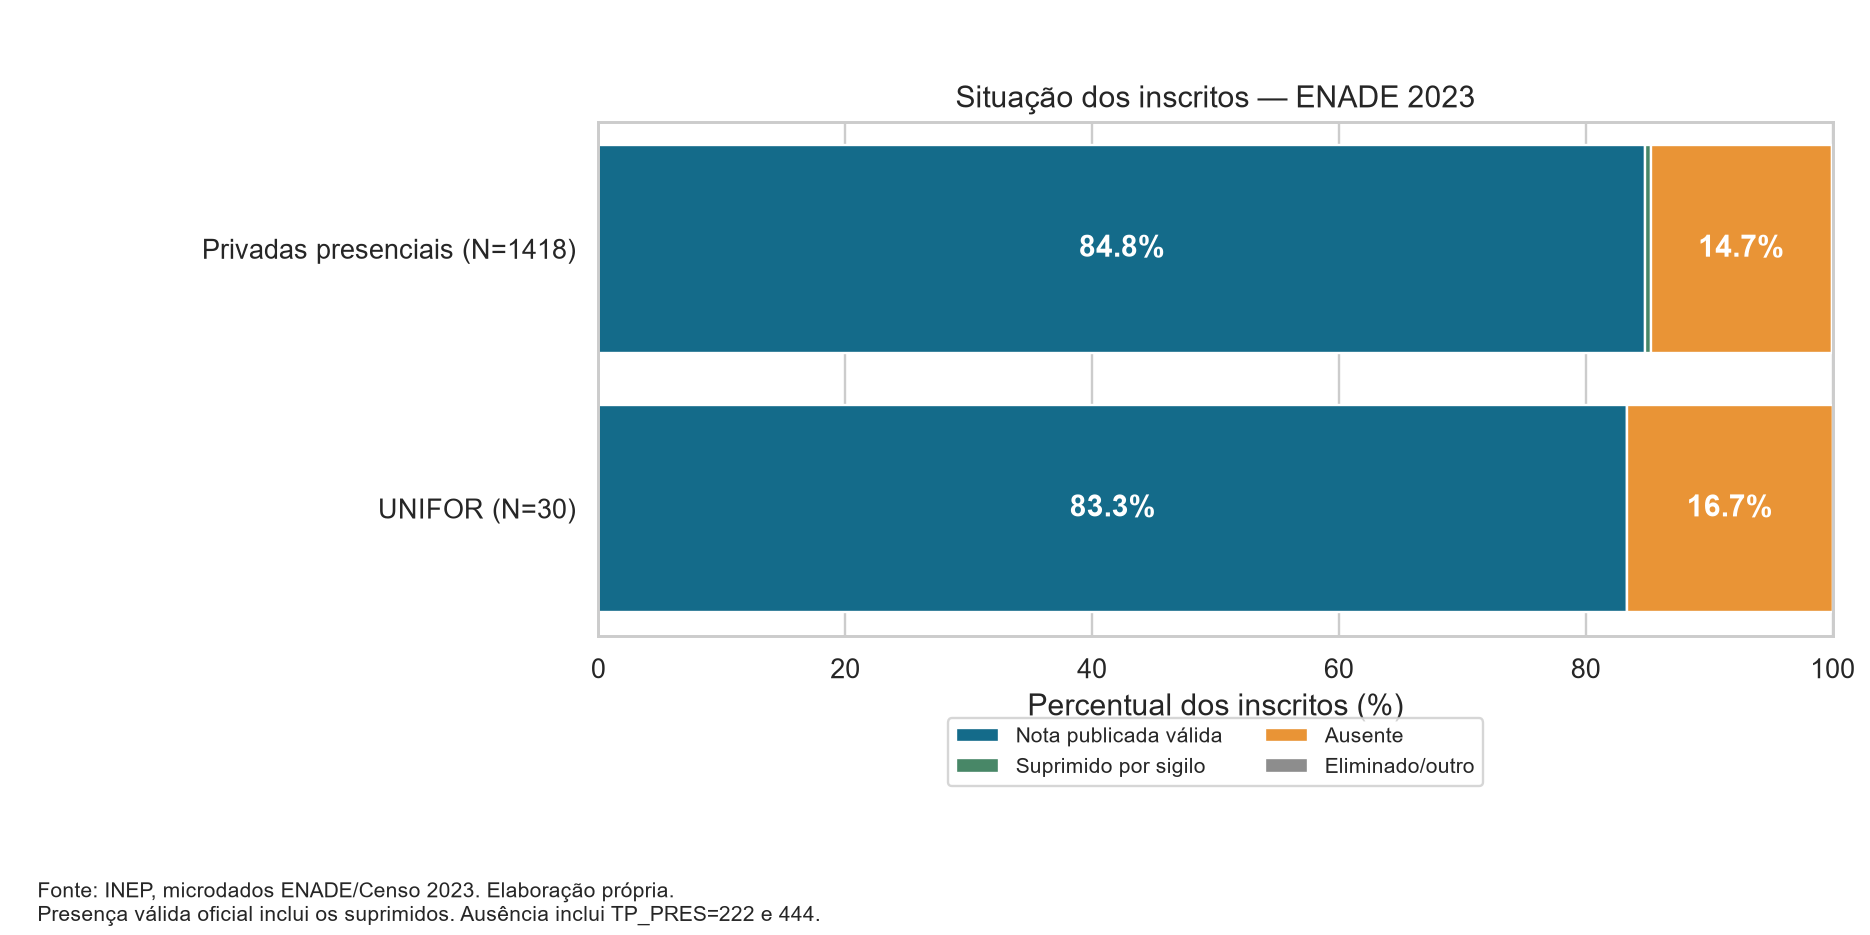
\includegraphics[width=\textwidth]{../resultados/graficos/participacao_2023.png}
\caption{Situação dos inscritos na UNIFOR e no universo privado presencial.
Fonte: INEP, ENADE/Censo 2023; elaboração própria.}
\label{fig:participacao}
\end{figure}

\subsection{Notas publicadas e distribuição}
A Tabela~\ref{tab:notas} apresenta os denominadores e a dispersão das três
notas. As Figuras~\ref{fig:distribuicao} e \ref{fig:medias} mostram suas
distribuições e médias. A densidade nos histogramas permite visualizar formatos
de distribuição com amostras de tamanhos diferentes; a UNIFOR integra o universo
privado usado como referência.

\begin{table}[htbp]
\centering\small
\caption{Estatísticas das notas brutas publicadas válidas, escala 0--100.}
\label{tab:notas}
\resizebox{\textwidth}{!}{\begin{tabular}{llrrrr}
\toprule
Grupo & Nota & n & Média & Mediana & DP amostral \\
\midrule
UNIFOR & Geral & 25 & 41,656 & 41,200 & 9,301 \\
UNIFOR & FG & 25 & 47,776 & 50,600 & 12,374 \\
UNIFOR & CE & 25 & 39,600 & 38,000 & 10,721 \\
Privadas presenciais & Geral & 1203 & 39,326 & 38,600 & 11,985 \\
Privadas presenciais & FG & 1203 & 51,550 & 51,200 & 15,946 \\
Privadas presenciais & CE & 1203 & 35,234 & 33,800 & 13,496 \\
Sem fins lucrativos & Geral & 676 & 42,440 & 41,800 & 11,749 \\
Sem fins lucrativos & FG & 676 & 52,737 & 52,800 & 15,931 \\
Sem fins lucrativos & CE & 676 & 38,989 & 37,800 & 13,233 \\
Universidades privadas & Geral & 521 & 38,164 & 37,500 & 11,820 \\
Universidades privadas & FG & 521 & 50,505 & 50,100 & 15,766 \\
Universidades privadas & CE & 521 & 34,033 & 33,800 & 13,411 \\
\bottomrule
\end{tabular}
}
\par\smallskip\footnotesize Fonte: INEP, ENADE/Censo 2023; elaboração própria.
FG: Formação Geral; CE: Componente Específico; DP: desvio-padrão amostral.
Cada linha usa exatamente $n$ notas; ausentes e suprimidos não entram nos cálculos.
\end{table}

\begin{figure}[htbp]
\centering
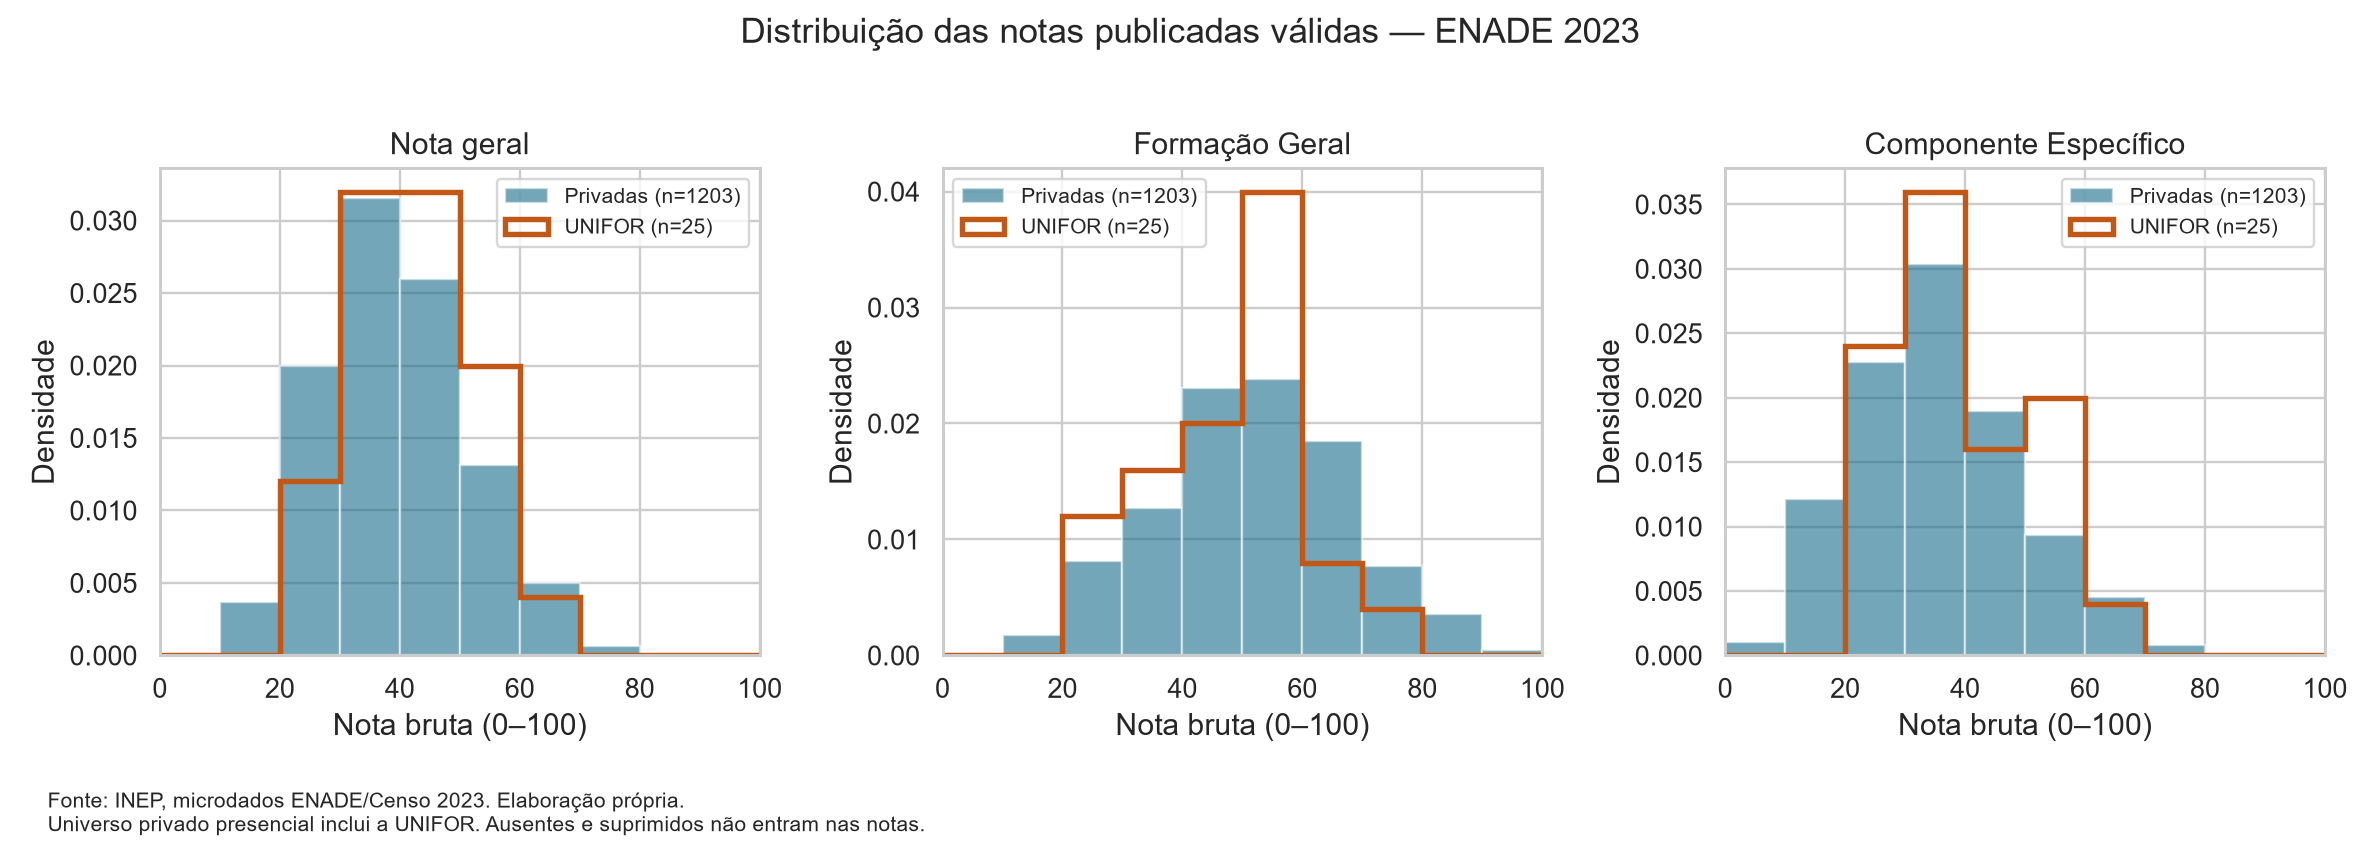
\includegraphics[width=\textwidth]{../resultados/graficos/distribuicao_notas_2023.png}
\caption{Distribuições das notas publicadas válidas. Fonte: INEP,
ENADE/Censo 2023; elaboração própria.}
\label{fig:distribuicao}
\end{figure}

\begin{figure}[htbp]
\centering
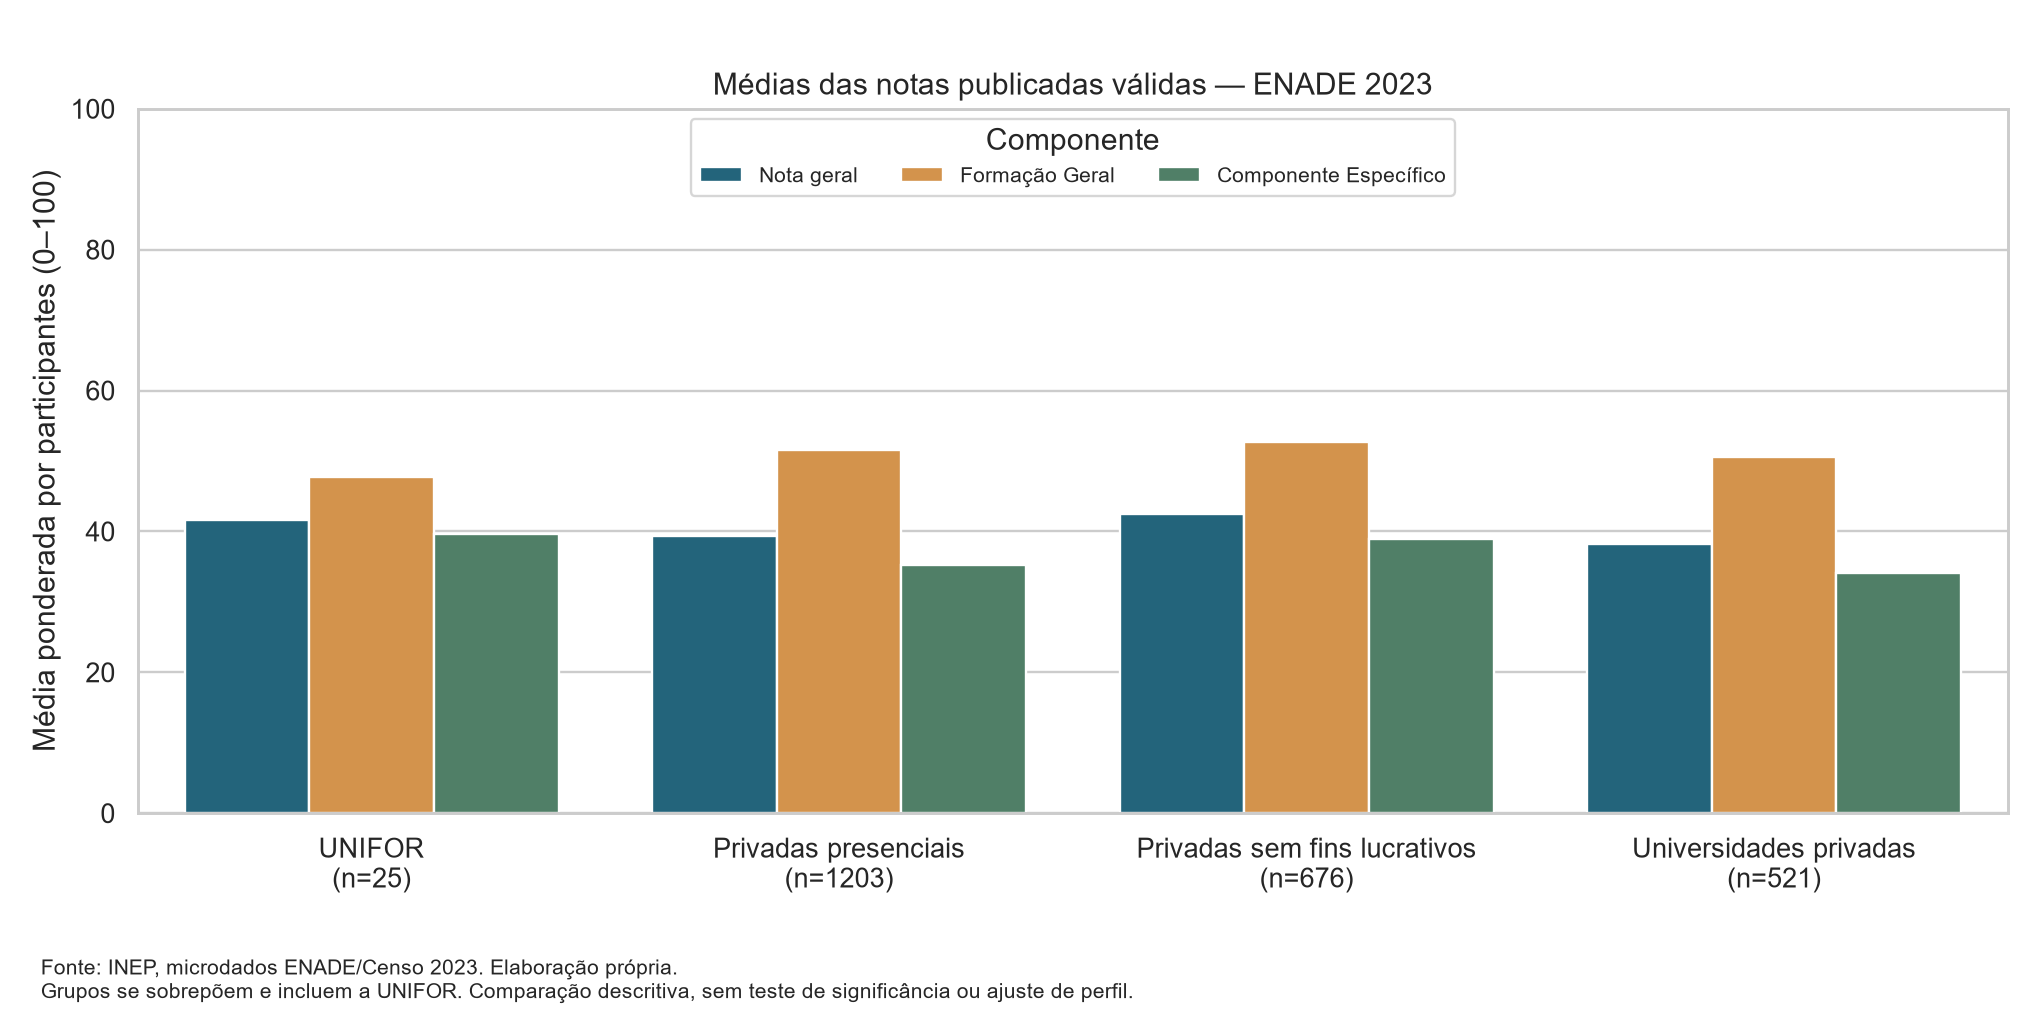
\includegraphics[width=\textwidth]{../resultados/graficos/medias_grupos_2023.png}
\caption{Médias por participante nos grupos de comparação. Fonte: INEP,
ENADE/Censo 2023; elaboração própria. Grupos incluem a UNIFOR.}
\label{fig:medias}
\end{figure}

\subsection{Dispersão e ponderação entre cursos}
A Figura~\ref{fig:dispersao} destaca apenas os \CursosDestaque{} cursos com
pelo menos dez notas válidas. O tamanho das amostras varia, o que limita a
interpretação de diferenças pontuais. Os cursos menores continuam nas tabelas
gerais. A média geral ponderada do universo é \MediaPrivadasGeral{}, enquanto
a média com peso igual por curso é \MediaCursosGeral{}. A diferença mostra
que resumir participantes e resumir cursos responde a perguntas distintas.

\begin{table}[htbp]
\centering\small
\caption{Média geral por participantes e com peso igual entre cursos.}
\label{tab:ponderacao}
\resizebox{\textwidth}{!}{\begin{tabular}{lrrrr}
\toprule
Grupo & Cursos com nota & Ponderada & Igual por curso & Igual, $n\geq10$ \\
\midrule
UNIFOR & 1 & 41,656 & 41,656 & 41,656 \\
Privadas presenciais & 71 & 39,326 & 38,005 & 39,535 \\
Sem fins lucrativos & 34 & 42,440 & 40,761 & 42,366 \\
Universidades privadas & 28 & 38,164 & 38,913 & 39,739 \\
\bottomrule
\end{tabular}
}
\par\smallskip\footnotesize Fonte: INEP, ENADE/Censo 2023; elaboração própria.
A última coluna restringe o cálculo aos cursos com $n\geq10$; as demais usam
todos os cursos com notas publicadas, inclusive amostras menores.
\end{table}

\begin{figure}[htbp]
\centering
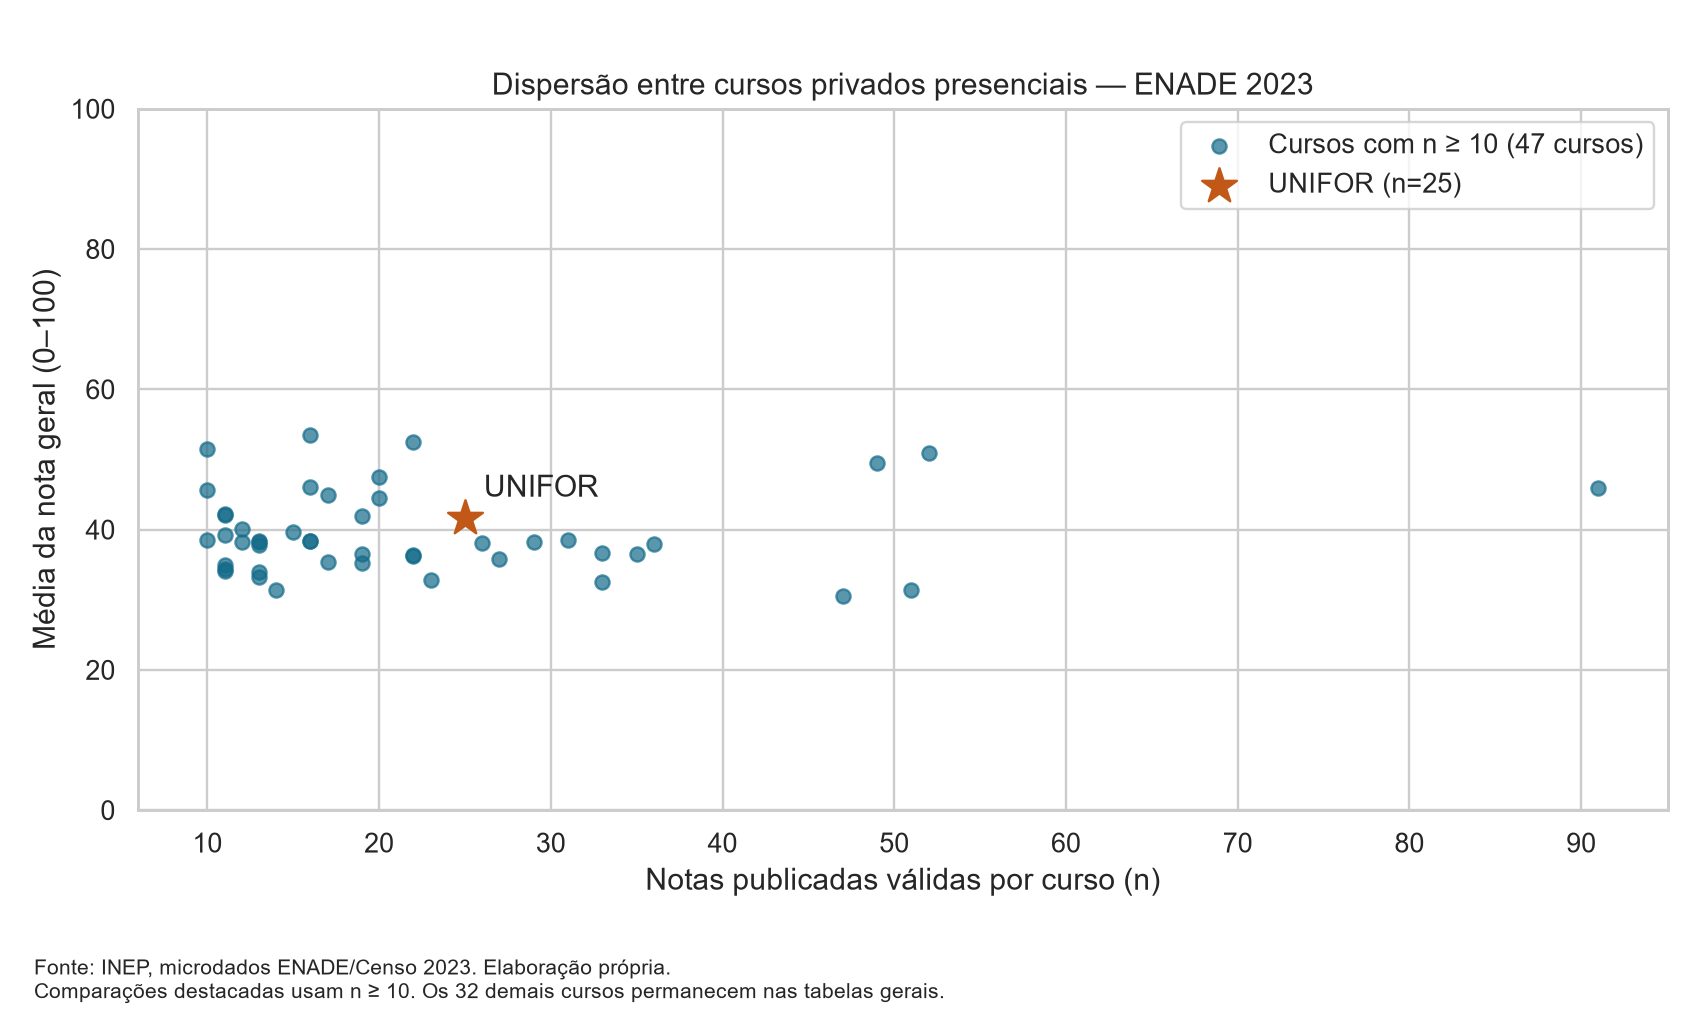
\includegraphics[width=.95\textwidth]{../resultados/graficos/dispersao_cursos_2023.png}
\caption{Dispersão das médias gerais e tamanhos das amostras de cursos com
$n\geq10$. Fonte: INEP, ENADE/Censo 2023; elaboração própria.}
\label{fig:dispersao}
\end{figure}

\section{Resultados e discussão}
A média geral da UNIFOR, \MediaUniforGeral{}, é maior que a média observada
do universo privado, \MediaPrivadasGeral{}. No recorte sem fins lucrativos,
a referência é \MediaSemFinsGeral{}, acima da média da UNIFOR; nas universidades
privadas, é \MediaUniversidadesGeral{}. A relação depende, portanto, do grupo
comparativo escolhido. A FG da UNIFOR é menor que a dos três grupos, enquanto
seu CE é maior, conforme a Tabela~\ref{tab:notas}.

Como verificação descritiva adicional, retirando a UNIFOR do universo privado
restam \NotasSemUnifor{} notas, com média geral \MediaSemUniforGeral{}.
Esse cálculo está na tabela CSV de grupos e não transforma os subconjuntos
em grupos comparáveis por perfil. As diferenças não foram ajustadas por
composição dos estudantes, infraestrutura, currículo ou seleção de participantes.
Não foram realizados testes de significância, estimativas de efeito causal,
entrevistas ou rankings definitivos.

\section{Limitações metodológicas}
O curso ENADE 1125254, da IES 137, não foi localizado no cadastro de cursos
Censo 2023, mas sua instituição está presente. O Censo registra Engenharia de
Computação nessa IES sob código 1637080. Não há prova documental de equivalência
entre códigos; não se fez substituição por semelhança de nome. O curso elegível
permanece no universo, com atributos de curso Censo ausentes.

A mesma IES tem categoria ENADE 8, indicador comunitária zero e confessional
um. A condição estrita comunitária igual a um não se confirma nesse caso;
a permanência é compatível com a definição comunitária/confessional e com
categoria Censo 5. A ressalva está explicitamente marcada no cadastro.

As notas suprimidas não podem ser recuperadas e as médias descrevem somente
os resultados publicados. Diferenças na participação e amostras pequenas podem
alterar o perfil observado. O corte de dez notas é uma escolha inicial para
destaques, sem garantir precisão ou representatividade. A granularidade anônima
impede controlar características individuais que estejam em arquivos separados.

O arquivo de relatório recebido estava vazio, sem conteúdo acadêmico anterior
recuperável. Esta versão usa a instituição e a disciplina confirmadas no projeto;
autoria, identificação docente e normas específicas da entrega devem ser revistas
pelo grupo. Não há compilador LaTeX disponível no ambiente usado: foram feitas
verificações estáticas, mas paginação e aparência final do PDF exigem compilação
e revisão humana em uma instalação existente.

\section{Conclusões preliminares}
A preparação corrigida ampliou o universo para todas as categorias privadas
documentadas e separou ausência de supressão. As notas publicadas da UNIFOR
apresentam média geral e CE acima do universo privado agregado e FG abaixo dele;
a comparação com instituições sem fins lucrativos produz referência geral mais
alta que a UNIFOR. Esses resultados contextualizam a amostra observada e não
demonstram qualidade global, causalidade ou superioridade estatística.

O pipeline, o notebook executado e as tabelas oferecem base verificável para
revisão acadêmica. As próximas decisões devem considerar as ressalvas do cadastro,
o sigilo e a heterogeneidade dos cursos. Nenhuma análise de 2021 foi executada.

\clearpage
\begin{thebibliography}{9}
\bibitem{enade} INEP. \textit{Microdados do ENADE 2023}.
Arquivos e dicionário oficiais fornecidos no ZIP local. Disponível em:
\url{https://www.gov.br/inep/pt-br/acesso-a-informacao/dados-abertos/microdados/enade}.
\bibitem{censo} INEP. \textit{Microdados do Censo da Educação Superior 2023}.
Cadastros e dicionário oficiais fornecidos no ZIP local. Disponível em:
\url{https://www.gov.br/inep/pt-br/acesso-a-informacao/dados-abertos/microdados/censo-da-educacao-superior}.
\bibitem{manual} INEP. \textit{Manual do usuário -- Enade 2023}.
Documento integrante do ZIP oficial de microdados ENADE 2023, pp.~6--7.
\bibitem{conceito} INEP. \textit{Conceito Enade}. Portal institucional.
Disponível em:
\url{https://www.gov.br/inep/pt-br/areas-de-atuacao/pesquisas-estatisticas-e-indicadores/indicadores-de-qualidade-da-educacao-superior/conceito-enade}.
Consulta em 15 out. 2026.
\bibitem{notatecnica} INEP. \textit{Nota Técnica nº 6/2024: metodologia de
cálculo do Conceito Enade 2023}. Disponível em:
\url{https://download.inep.gov.br/educacao_superior/enade/notas_tecnicas/2024/nota_tecnica_6_metodologia_calculo_conceito_enade_2023.pdf}.
Consulta em 15 out. 2026.
\end{thebibliography}
\end{document}
